\documentclass[a4paper]{article}

\usepackage[english]{babel}
\usepackage[utf8]{inputenc}
\usepackage{amsmath}
\usepackage{graphicx}
\usepackage[colorinlistoftodos]{todonotes}
\usepackage{caption}
\usepackage{pgfplots}
\pgfplotsset{width=10cm,compat=1.9}
\renewcommand{\thetable}{\arabic{section}.\arabic{table}}
\newcommand\T{\rule{0pt}{2.6ex}}       % Top strut
\newcommand\B{\rule[-1.2ex]{0pt}{0pt}} % Bottom strut

\title{PHY 4210-01 Senior Lab \\Lab M-1: Magnetic Field Mapping}

\author{Sarah Arends \\ 
        Jacquelyne Miksanek \\
        Ryan Wojtyla \\ \\
        Instructor: Jerry Collins II}

\date{February 7, 2019}

\begin{document}
\maketitle 

\begin{abstract}
%physics of experiment
%apparatus used
%what was measured
\end{abstract}

\newpage

\tableofcontents

\newpage

\section{Objective of the Experiment}
%A brief statement on the main purpose of the experiment
During this lab, a 3-dimensional mapping of the magnetic field inside a Helmholtz coil was created in order to investigate the presence of a uniform field, running along the axial direction of the Helmholtz coil. 

\section{Theory of the Experiment}
%A short presentation of the concepts and formulas related to the experiment.

% How a helmholtz coil produces a uniform field
Recall for a straight current-carrying wire, circular magnetic field lines are generated around the wire in accordance with the curling right-hand rule. The Helmholtz coil contains two regions of circularly wound wires. Due to the the circular symmetry, all components of each infinitesimal segment of the wire will cancel \textit{except} for that in the axial direction. In summary, a circular current produces a linear magnetic field.

\section{Equipment Utilized}
%List principal pieces of apparatus used by manufacturer, model and serial number. When it may be important, list principal specifications of certain pieces of equipment (e.g. the focal length of an optical system, etc.)

%How hall effect probe works
A DC Gaussmeter (AlphaLab Model GM-1-HS) was connected to a Hall Effect Probe in order to measure the field strength inside the Helmholtz coil. The Hall Effect Probe contains a semiconductor junction that, when exposed to a magnetic field, produces a voltage proportional to the field strength.

%Position Controls
The position of the Hall Effect Probe can be modified in the $\rho$ direction by sliding the ruler bar through the acrylic cube shown in figure \ref{diagram}. The position can be modified in the $\phi$ direction by rotation the ruler bar about the central pole. However, for the sake of this experiment, this did not have to be modified because measurements were taken in a single $\rho , z$ plane. The $z$ coordinate was modified by sliding the acrylic cube and ruler bar up and down the central pole.

%Labeled sketch of the experimental setup
\begin{figure}[h]
\centering
% uncomment the line below to add image
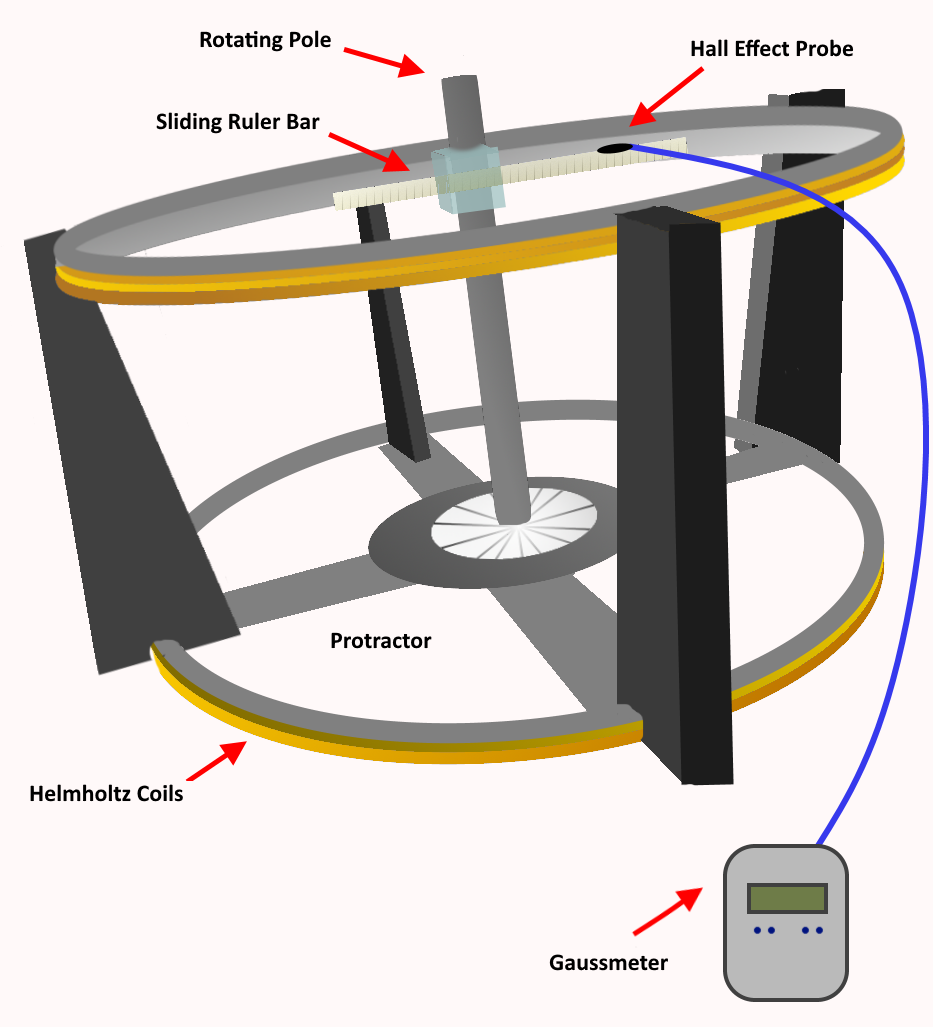
\includegraphics[width=0.5\textwidth]{helmholtz_diagram.png}
\captionof{figure}{Two concentric Helmholtz coils seperated by a distance equal to their radius. Rotating pole and sliding ruler allow for modification of the probe's position.}
\label{helmholtz_diagram}
\end{figure}


\section{Procedure}
% Describe in writing and provide a detailed sketch of the equipment used to measure the axial field in the coil.




%Describe the main steps in the experimental procedures. Be sure to include any precautions. Sufficient details should be given such that another student can follow and do the experiment.
Note that, per suggestion of the laboratory manual, the procedural steps of this experiment have been omitted. The discussion section provides sufficient detail on what actions were taken.

\subsection{Data Analysis}
%Graphs, figures, and tables with captions
%Results with error analysis
%Calculate discrepancies from theory

% Calculating

%Theoretical calculations of axial field strength

% 3D plot (theoretical)

% 2D plot (theoretical)

% 3D plot (exp)

% 2D plot (exp)

% Calculating discrepancies

% 3D plot discrepancies 

% 2D plot discrepancies

\section{Results}
%Discuss results and uncertainties
%Compare results with theory
%Approximations to theory


% Determine span of uniform region with 1percent margin and 5percent margin

% Compare B field in different direction, can we say field is axial

\section{Conclusion}
%Brief summary, discussion of results and theory

\end{document}